%***************************************************************************************************************************************************
\chapter[Sensitivity Analysis]{Sensitivity Analysis: Understanding Model Input/Output Relationship Under Uncertainty}\label{ch:gsa}
%***************************************************************************************************************************************************

% Linking Paragraph
As mentioned in the introduction, describing and understanding properly the impact of model parameters variations on the model prediction are an essential part of the model development and assessment. 
This chapter presents the application of global and statistical \gls[hyper=false]{sa} to analyze the \gls[hyper=false]{feba} model in \gls[hyper=false]{trace} in order to investigate the effects of the input parameter variations.

% Focus
After first introducing in Section~\ref{sec:sa_statistical_framework} the notational convention used in the present chapter,
the proposed methodology is presented.
The methodology leverages various developments in global \gls[hyper=false]{sa} and \glsfirst[hyper=false]{fda} methods and follows three key underlying ideas.

% Overview
The first idea, presented in Section~\ref{sec:sa_time_dependent_variation}, is to reduce the dimensionality of the output space while preserving the interpretability of the results by utilizing techniques derived from \gls[hyper=false]{fda} \cite{Ramsay2005}.
Section~\ref{sec:sa_parameters_screening} introduces the second idea, which is to reduce the dimensionality of the input parameter space through screening analysis using the Morris method \cite{Morris1991,Campolongo2011}. 
The third and final idea is to investigate, quantitatively and in more detail, the effect of variation of parameters on the overall time-dependent output variation. 
This is done through variance-based SA using the Sobol’-Saltelli
method \cite{Sobol2001, Saltelli2002}, which is presented in Section~\ref{sec:sa_variance_decomposition}.

The methods are then applied to analyze the \gls[hyper=false]{feba} model in \gls[hyper=false]{trace} to understand better its inputs/outputs relationship under the assumed uncertainty on its input parameters.
The results are presented and discussed in Section~\ref{sec:sa_application_to_feba}.
Finally, Section~\ref{sec:sa_chapter_summary} closes the chapter with a summary.

%%******************************************************************
\section{Statistical Framework}\label{sec:gp_statistical_framework}
%******************************************************************

Consider a general \emph{regression} problem:
\marginpar{regression problem}
Given a deterministic computer simulator (which, in essence, is a function) $f:\mathbf{x} \in \mathcal{X} \subseteq \mathbb{R}^D \mapsto \mathbb{R}$ 
evaluated at $\mathbf{DM}$, an experimental design matrix $\{\mathbf{x}_n\}_{n=1}^N$,
yielding $N$ outputs $\mathbf{y} = \{f(\mathbf{x}_n) = y_n\}_{n=1}^N$. 
the objective of regression is to compute (or \emph{predict}) the value of $f(\mathbf{x}_o)$ with $\mathbf{x}_o \notin \mathbf{DM}$.

The set $\mathcal{D} \equiv \{(\mathbf{DM}, \mathbf{y})\} = \{(\mathbf{x}_n, f(\mathbf{x}_n) = y_n)\}_{n=1}^N$ of $N$ observations is often referred to as the training data,
\marginpar{training data, training samples, and training outputs}
though the term is used interchangeably with the training outputs $\mathbf{y}$.
The experimental design matrix $\mathbf{DM}$ introduced in the previous chapter is interchangeably referred to as the training samples, inputs, or points in this chapter.
As before, the domain $\mathcal{X}$ is often rescaled such that $\mathbf{x} \in [0,1]^D$.

To evaluate $f$ at any given $\mathbf{x}_o \notin \mathbf{DM}$, the code of course can be simply run at that input.
\marginpar{emulator, surrogate model, and metamodel} 
Unfortunately, the true underlying function $f(\circ)$ that produces $y_i$ itself might be too complex and expensive to evaluate.
As such, the response surface of the function has to be reconstructed or estimated based only on small size of training data before the prediction is made.
The estimated function is chosen to be a simpler function that can be evaluated much faster (such as polynomials).
Although simpler, such an approximation should capture the most, if not all, important aspects of the inputs/outputs relationship of the true underlying function.
This simpler, approximating function is often referred to as an \emph{emulator}, \emph{surrogate model}, or \emph{metamodel}.

% Adopted framework
In this thesis, 
\marginpar{Gaussian process metamodel}
the metamodel is represented using \gls[hyper=false]{gp}, following the seminal works of Sacks et al. (\cite{Sacks1989, Sacks1989a}) and interpreted through a Bayesian perspective.
The advantages of using \gls[hyper=false]{gp} to represent an unknown function are its ability to model a complicated multi-dimensional function with limited number of parameters (\cite{Jones2009})
as well as the provision of prediction error estimate (\cite{Santner2003,Currin1991}).
Furthermore, being a statistical model based on a stochastic process, it fits the statistical calibration framework of computer model presented in the next chapter.

% Two Interpretations
The \gls[hyper=false]{gp} metamodel, like many statistical models, can be interpreted either in frequentistic sense or Bayesian sense.
\marginpar{Two interpretations}
In the frequentistic sense, the stochastic process $Y(\circ)$ is one particular realization of stochastic process (need not be Gaussian, but second-order stationary).
The prediction made at particular value of $\mathbf{x}_o$ is made based on the process as estimated according to the training data\footnote{The frequentistic case is the classical approach first developed as spatial interpolation tool in geostatistics by Krige dating back to the 1950s \cite{Krige1951} and formalized by Matheron in the 1960s \cite{Matheron1963}. In fact, Kriging model (due to Krige) is the more popular term for \gls[hyper=false]{gp} metamodel. These two terms, Kriging model and \gls[hyper=false]{gp} metamodel, will be used interchangeably in this thesis.}.
On the other hand, in the Bayesian sense, a Gaussian process is first set up as the prior for the stochastic process and the
prediction of the output at $\mathbf{x}_o$ is made based on the posterior (or conditional) process as updated by the training data.   

Both of these interpretations give an equivalent results.
The subtle difference lies in the interpretation of prediction error.
In the frequentistic case, the error is defined as the mean squared of error between the prediction made by the estimated process and (hypothetical) true process \cite{Isaaks1989};
\marginpar{prediction error}
while in the Bayesian case the error corresponds to the \emph{epistemic} uncertainty of the prediction conditional on the observed data.
That is, though the underlying computer simulation itself might be deterministic, 
the uncertainty of the prediction at $\mathbf{x}_o$ stems from the fact that the simulator was not actually run at that input and thus the output is not \emph{known}. 
The Bayesian perspective, as argued in \cite{Currin1991,Santner2003,OHagan2006}, gives more intuitive interpretation of the prediction error.
This perspective is illustrated in Fig.~\ref{fig:plot_bayesian_perspective}.
\bigtriplefigure[pos=tbhp,
								 mainlabel={fig:plot_bayesian_perspective},
			           maincaption={Gaussian process prior is equivalent to setting prior over functions. After observing data the process is updated to obtain the posterior process with a reduced uncertainties. Uncertainties are attached to each prediction made at arbitrary input outside the data (red points). Dashed lines and gray region signify the mean and $3\times \sigma$, respectively. The scales in the axes are arbitrary.},
			           mainshortcaption={Illustration of Bayesian perspective of regression and metamodeling.},%
			           leftopt={width=0.30\textwidth},
			           leftlabel={fig:plot_bayesian_perspective_1},
			           leftcaption={Prior of functions},
			           midopt={width=0.30\textwidth},
			           midlabel={fig:plot_bayesian_perspective_2},
			           midcaption={Observed data},
			           rightopt={width=0.30\textwidth},
			           rightlabel={fig:plot_bayesian_perspective_3},
			           rightcaption={Posterior function and predictions},
			           spacing={},
			           spacingtwo={}]
{../figures/chapter4/figures/plotBayesianPerspective_1}
{../figures/chapter4/figures/plotBayesianPerspective_2}
{../figures/chapter4/figures/plotBayesianPerspective_3}

%\section{Describing Variation of Time-Dependent Output}\label{sec:sa_time_dependent_variation}
Illo principalmente su nos. Non message \emph{occidental} angloromanic
da. Debitas effortio simplificate sia se, auxiliar summarios da que,
se avantiate publicationes via. Pan in terra summarios, capital
interlingua se que. Al via multo esser specimen, campo responder que
da. Le usate medical addresses pro, europa origine sanctificate nos
se.
%%****************************************************************
\section{Parameters Screening}\label{sec:sa_parameters_screening}
%****************************************************************

Screening methods are used to rank the importance of the model parameters using a relatively small number of model evaluations \cite{Saltelli2004}.
However, they tend to simply give qualitative measures.
That is, meaningful information resides in the rank itself but not in the exact importance of the parameters with respect to the output. 
Screening is particularly valuable in the early phase of a SA to identify the noninfluential parameters of a model,
which then could be safely excluded from further detailed analysis. 
This step is important to reduce the size of the problem especially if more expensive methods are to be applied at the subsequent steps. 
In this work, attention was paid to a particular screening method proposed by Morris \cite{Morris1991} with an extension proposed by Campolongo et al. \cite{Campolongo2011}.

%----------------------------------------------------------------------------
\subsection{Elementary Effects and One-at-a-Time Design}\label{sub:sa_ee_oat}
%----------------------------------------------------------------------------

% Elementary effect definition
Consider a mathematical model $f: \bm{x} \in [0,1]^D \mapsto y = f(\bm{x}) \in \mathbb{R}$, 
where $\bm{x} = (x_1, x_2, \dots,x_D)$ is a vector of input parameters.
The elementary effect of the $d$-th parameter on $f$ is defined as
\marginpar{elementary effect}
\begin{equation}
  EE_d = \frac{f(x_1, \dots, x_d+\Delta,\dots,x_D) - f(x_1, \dots, x_d,\dots,x_D)}{\Delta}
\label{eq:elementary_effect}
\end{equation}
or more concisely,
\begin{equation}
  EE_d = \frac{f(\bm{x} + \Delta \cdot \bm{e}_d) - f(\bm{x})}{\Delta}
\label{eq:elementary_effect_concise}
\end{equation}
where $\bm{e}_d$ is the $d$-th basis vector of the input parameter space;
and $\Delta$, the grid jump, is chosen such that $\mathbf{x} + \Delta \cdot \bm{e}_d$ is still in the specified domain of the parameter space, i.e., $[0,1]^D$; 
$\Delta$ is a value in $\{\frac{1}{p-1}, \dots, 1 - \frac{1}{p-1}\}$, 
where $p$ is the number of (discretization) levels that partition the model parameter space into a uniform grid of points where the model can be evaluated. 
For a given $p$, the grid constructs a finite distribution of $p^{D-1}[p - \Delta(p-1)]$ elementary effects for each input parameter.

% OAT Experimental Design
The elementary effect distributions for each of the input parameters,
evaluated across discretized input parameter space, 
\marginpar{\gls[hyper=false]{oat} experimental design}
provide useful information on the importance of a parameter on the output.
Unfortunately, an exhaustive evaluation of all elementary effects for a given discretization levels suffers from a curse of dimensionality especially for numerous parameters and/or for reasonably fine discretization level\footnote{for $p = 8$ and $D = 20$ the total number of evaluations for exhaustive computation of all $EE$s is $\approx 6 \times 10^{17}$ for each parameter}.
Consequently, a class of design of experiment that only change one parameter at a time (\gls[hyper=false]{oat}) are devised to estimate the statistics of the distributions.
  
% Trajectory OAT Design
The key idea behind the original Morris method is in initiating the model evaluations from various \textit{nominal} points, $\bm{x}$,
\marginpar{trajectory OAT design}
randomly selected over the grid and then gradually advancing one grid jump, perturbing one parameter at a time,
making a perturbed point as the base point for the next perturbation.
The order of perturbation (i.e., which dimension to perturb first) and the direction of the perturbation (i.e., whether it is added or subtracted) are also randomized between replications.
As such, different replication generates different starting nominal point as well as different order and sign (but with the same size) of perturbation.
The \gls[hyper=false]{oat} experimental design complemented with this requirement is known as the trajectory design \cite{Ruano2012}.
Fig.~\ref{fig:ch3_plot_oat_illustration_1} illustrates a trajectory design with $4$ replications in a two-dimensional input parameter space discretized in $6$ levels .
\normdoublefigure[pos=tbhp,
                  mainlabel={fig:ch3_plot_oat_illustration},
                  maincaption={Illustration of One-at-a-Time (OAT) design constructed using trajectory scheme (left) and radial scheme (right) each with 4 replications. The trajectory design is discretized in 6 levels, while the number of levels is irrelevant for radial design. Filled circles are the nominal or the starting point (for the trajectory) or the base (for the radial) points and crosses are the perturbed levels.},%
									mainshortcaption={Illustration of One-at-a-Time (OAT) design using trajectory and radial schemes.},
                  leftopt={width=0.45\textwidth},
                  leftlabel={fig:ch3_plot_oat_illustration_1},
                  leftcaption={Trajectory scheme},
                  %leftshortcaption={},%
                  rightopt={width=0.45\textwidth},
                  rightlabel={fig:ch3_plot_oat_illustration_2},
                  rightcaption={Radial scheme},
                  %rightshortcaption={},
                  %spacing={\hfill}
                 ]
{../figures/chapter3/figures/plotOATIllustration_1}
{../figures/chapter3/figures/plotOATIllustration_2}

To remove the requirement to specify a method-specific parameter $p$ (the number of levels),
\marginpar{radial OAT design}
Campolongo et al.\cite{Campolongo2011} proposed to use a radial scheme coupled with Sobol' quasirandom sequence.
In a single replication of this particular OAT design, 
each parameter is perturbed relative to a \textit{base/nominal} point 
which is not required to be located on a predetermined grid.
The size and sign of the perturbation is also allowed to vary from parameter to parameter in different replication.
As such, radial design implicitly incorporates several additional possible sources of variation in the method 
that can potentially bias the estimation of elementary effects.
Because the size of parameter perturbations varies, the definition of the elementary effects is slightly changed to,
\marginpar{elementary effect for radial design}
\begin{equation}
EE_d = \frac{f(\bm{x} + \Delta x_d \cdot \bm{e}_d) - f(\bm{x})}{\Delta x_d}
\end{equation}
where now each parameter at each design replication has its corresponding perturbation size $\Delta x_d \in [-1,1]$ such that $x_d + \Delta x_d \in [0,1]$.

An illustration of a radial design in a two-dimensional input parameter space with $4$ nominal/base points is shown in Fig.~\ref{fig:ch3_plot_oat_illustration_2}.
 
%-------------------------------------------------------------------------------------------------
\subsection{Statistics of Elementary Effects and Sensitivity Measures}\label{sub:sa_ee_statistics}
%-------------------------------------------------------------------------------------------------

% Mean of the elementary effects
Consider now that an $N_R$ number of elementary effects associated with the $d$-th parameter have been sampled from the finite distribution of $EE_d$,
using a \gls[hyper=false]{oat} design with $N_R$ replications.
The statistical summary of sampled $EE_d$ based on a given number of OAT design replications generated using either the trajectory or the radial design can be calculated.
The first is the arithmetic mean defined as,
\marginpar{the mean of the (sampled) elementary effects}
\begin{equation}
	\mu_d = \frac{1}{N_R} \sum_{r = 1}^{N_R} EE^r_d
	\label{eq:sa_morris_mu}
\end{equation} 
where $EE^r_d$ is the elementary effect of the $d$-th parameter of the $r$-th replication.
The mean gives the global influence of the $d$-th parameter on the chosen output $f$.

% Standard deviation of the elementary effects
The second statistical summary of interest is the standard deviation of the (sampled) elementary effects for input parameter $x_d$,
\marginpar{the standard deviation of the (sampled) elementary effects}
\begin{equation}
	\sigma_d = \sqrt{\frac{1}{N_R} \sum_{r = 1}^{N_R} (EE^r_d - \mu_d)^2}
	\label{eq:sa_morris_sd}
\end{equation} 
The standard deviation gives an indication of the presence of nonlinearity and/or interactions between the $d$-th input parameter and the others.

% Mean of absolute values of the elementary effects
In cases where $f$ is a non-monotonic function,
the sign of $EE_d$ may change according to the change of the output,
and cancellation effects on the estimation of $\mu_d$ might occur .
To circumvent this issue,
Campolongo et al.~\cite{Campolongo2011} proposed to take the absolute values of the sampled elementary effects.
It is defined as,
\marginpar{the mean of the (sampled) absolute elementary effects}
\begin{equation}
	\mu^*_d = \frac{1}{N_R} \sum_{r = 1}^{N_R} |EE^r_d|
	\label{eq:sa_morris_mustar}
\end{equation}
Note that although the overall sign of the output perturbation is lost by using this measure,
its use is justified if the input parameters are to be ranked based on a single importance measure.

% Interpretation and importance classification
The aforementioned statistical summaries, when evaluated over a large number of replications $N_R$,
can provide global sensitivity measures of the importance of each input parameter.
\marginpar{input parameter importance classification}
As indicated by Morris \cite{Morris1991}, there are three possible categories of parameter importance based on those statistics:
\begin{enumerate}
	\item Parameters with noninfluential effects, i.e., the parameters that have relatively small values of both $\mu_d$ (or $\mu^*_d$) and $\sigma_d$;
	The parameter has a negligible overall effect on the model output.
	\item Parameters with linear and/or additive effects, i.e., the parameters that have relatively large value of $\mu_d$ (or $\mu^*_d$) and relatively small value of $\sigma_d$.
	The small value of $\sigma_d$ and the large value of $\mu_d$ (or $\mu^*_d$) indicate that the variation of elementary effects across replications is small while the magnitude of the effect itself is consistently large for the perturbations in the parameter space.
	\item Parameters with nonlinear and/or interaction effects, i.e., the parameters that have a relatively small value of $\mu_d$ (or $\mu^*_d$) and a relatively large value of $\sigma_d$.
	Opposite to the previous case, a small value of $\mu_d$ (or $\mu^*_d$) indicates that the aggregate effect of perturbation is relatively small (or in the case of $\mu_d$, can be close to zero) while a large value of $\sigma_d$ indicates that the variation of the effect is large; the effect can be large or negligibly small depending on the values of the other parameters at which the model is evaluated.
	Such large variation is a symptom of nonlinear effects and/or parameter interaction.
\end{enumerate}

% Classification and qualitative measure
Such classification makes parameter importance ranking and, in turn, screening of noninfluential parameters possible.
However, the procedure is done rather qualitatively, and this is illustrated in Fig.~\ref{fig:ch3_importance_classification}, 
which depicts a typical parameter classification derived from visual inspection of the elementary effects statistics on the $\sigma$ vs. $\mu^*$ plane.
The notions of influential and noninfluential parameters are based on the relative locations of those statistics in the plane.
Typically, the noninfluential ones are clustered closer to the origin (relative to the more influential ones) with a pronounced boundary such as the one depicted in Fig.~\ref{fig:ch3_importance_classification}. 
Admittedly, if these statistics are spread somewhat uniformly across the plane, 
the distinction would be more ambiguous and problematic\footnote{In such a case, a more advanced classification such as the ones based on clustering techniques might be helpful to identify a finer structure of the parameters importance.}.
Furthermore, for a parameter with a large value of both $\mu^*$ and $\sigma$,
the method cannot distinguish between nonlinearity effect from parameter interaction effect on the output.

\begin{figure}[bth]
	\centering
	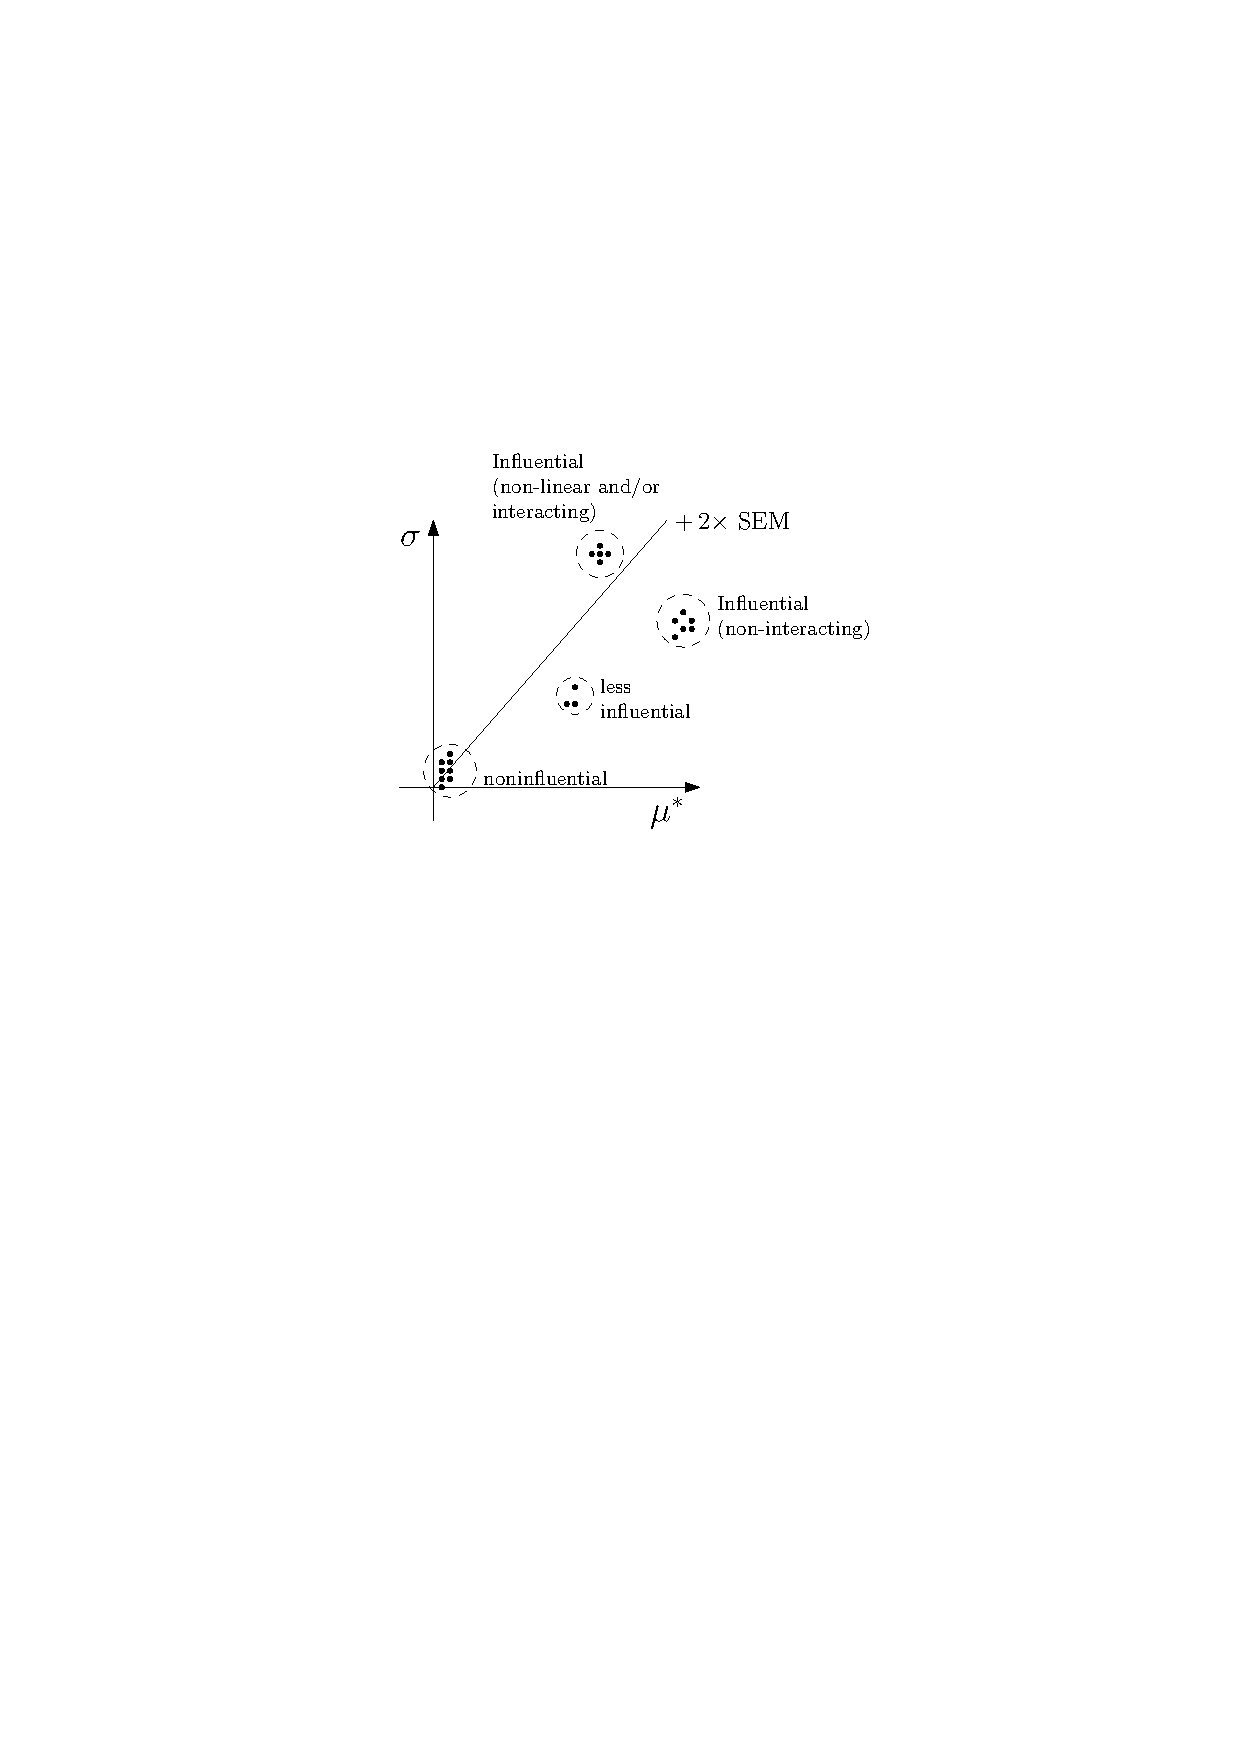
\includegraphics[scale=0.80]{../figures/chapter3/ipe/importance_classification}
	\caption[Illustration of a typical parameter importance classification based on Morris screening method]{Illustration of a typical parameter importance classification obtained from the Morris screening method. The importance of each parameter relative to the other ones is defined with respect to its location on the $\sigma - \mu^*$ plane. Each dot represents a parameter, and the line corresponds to twice the standard error of the mean (SEM) indicating the relative magnitude of the standard deviation to the mean.}\label{fig:ch3_importance_classification}
\end{figure}

%\section{Variance Decomposition}\label{sec:variance_decomposition}
Illo principalmente su nos. Non message \emph{occidental} angloromanic
da. Debitas effortio simplificate sia se, auxiliar summarios da que,
se avantiate publicationes via. Pan in terra summarios, capital
interlingua se que. Al via multo esser specimen, campo responder que
da. Le usate medical addresses pro, europa origine sanctificate nos
se.
%\section{Implementation}\label{sec:sa_implementation}

An implementation of the Morris method and a Monte Carlo method to estimate the main- and total-effect sensitivity indices has been developed using the Python \cite{PCT2017} programming language 
for the purpose of this work, to allow for well-controlled parametric and convergence studies.
The implementation follows a black box approach of sensitivity analysis. 
It deals with the generation of design of experiment (which is used to evaluate the model or code) and the post-processing of output to obtain the select measures of sensitivity.
In the following, the basic procedures that underlie the implementation of both methods are laid out.
More details on the programming aspects of the implementation (the so-called \texttt{gsa-module}) can be found in Appendix~\ref{app:gsa_module}.

\subsection{The Morris Method}\label{sub:sa_morris}

The implementation of the Morris method (see Section~\ref{sub:sa_ee_oat}) follows four sequential steps. 
\textsc{First}, an OAT design matrix consisting of $N_R$ replications is created by randomly sampling the nominal (base) points as well as the perturbed points for each parameter.
A replication in an OAT design consists of $1$ nominal point with $D$ (number of dimen~sions/parameters) additional perturbed points.
In each of the perturbed points, only one parameter change its value relative to the base.
Different replication yields different nominal point and the associated perturbed points.

\textsc{Second}, each point in the design matrix is scaled to the corresponding point in the $D$-dimensional parameter space of the model parameters.

\textsc{Third}, the model is evaluated for each (rescaled) point in the design matrix. The total number of model evaluations for a given design matrix of size $N_R$ is $N_R \times (D + 1)$.

\textsc{Fourth} and finally, the $N_R$ elementary effects $EE_d$ for each parameter and each trajectory are computed for a selected \gls{qoi}.
Their statistical summaries ($\mu_d$, $\mu_d^*$, $\sigma_d$) are then computed, 
and the ranking of the parameters can be constructed based on $\mu_d^*$ for a selected \gls{qoi}.
The $\mu_d^*$ can be directly used to rank the parameters to systematically identify 
and screen out noninfluential parameters (low $\mu_d^*$) from the relatively influential ones (high $\mu_d^*$)~\cite{Campolongo2007}.

\subsection{The Sobol'-Saltelli Method}\label{sub:sa_sobol_saltelli}

In principle, the estimation of the Sobol' indices defined by Eqs.~(\ref{eq:sa_main_effect_index}) and (\ref{eq:sa_total_effect_index}) can be directly carried out using \gls{mc} simulation.
\marginpar{brute force \\ Monte Carlo}
The most straightforward, though rather naive, 
implementation of \gls{mc} simulation to conduct the estimation is using two nested loops for the computation of the conditional variances and expectations appearing in both equations.

In the estimation of the main-effect index of parameter $x_d$, for instance, 
the outer loop samples values of $X_d$ while the inner loop samples values of $\mathbf{X}_{\sim d}$ (anything else other than $x_d$).
These samples, in turn, are used to evaluate the model output.
In the inner loop, the mean of the model output (for a given value of $X_d$ but over many values of $\mathbf{X}_{\sim d}$) is taken. 
Afterward, in the outer loop, the variance of the model output (over many values of $X_d$) is taken.
This approach can easily become prohibitively expensive as the nested structure requires $N^2$ model evaluations \emph{per input dimension} for either the main-effect and total-effect indices, 
while $N$ (the size of \gls{mc} samples) are typically in the range of $10^2 - 10^4$ for a reliable estimate. 

Sobol' \cite{Sobol2001} and Saltelli \cite{Saltelli2002} proposed an alternative approach that circumvent the nested structure of \gls{mc} simulation to estimate the indices.
The formulation starts by expressing the the expectation and variance operators in their integral form 
and ends with different possible \gls{mc} estimators for both sensitivity indices.
A detailed derivation of the integral form and the origin of the estimator can be found in Appendix~\ref{app:sobol_saltelli}. 

The computational cost associated with the estimation of all the main-effect and total-effect indices using the Sobol'-Saltelli method is $N \times (D + 2)$ code runs,
\marginpar{computational cost: \\ brute force Monte Carlo vs. Sobol'-Saltelli}
where $N$ is the number of \gls{mc} samples and $D$ is the number of parameters.
Compare this to the cost of brute force Monte Carlo of $2 \times D \times N^2$ code runs to estimate all the main-effect and total-effect sensitivity indices. 

As an additional comparison, the cost for Morris method to compute the statistics of elementary effect is $N_R \times (D + 1)$ code runs,
\marginpar{computational cost: \\ Morris vs. Sobol'-Saltelli}
where $N_R$ is the number of OAT design replications.
In either methods, the number of samples $N$ (in the case of the Sobol'-Saltelli method) and replications $N_R$ (in the case of the Morris method)
determines the precision of the estimates.
A larger number of samples (and replications) increases the precision.
Note, however, that in practice the typical number of Morris replications is between $10^1 - 10^2$~\cite{Saltelli2010}, 
while the number of \gls{mc} samples for the Sobol' indices estimation amounts to $10^2 - 10^4$~\cite{Sobol2001}.

As it was the case for the Morris method, an implementation of the Sobol'-Saltelli method is also part of \texttt{gsa-module} python3 package (see Appendix~\ref{app:gsa_module} for detail). 
For $N$ number of \gls{mc} samples and $D$ number of model parameters, the \gls{mc} simulation procedure to estimate the sensitivity indices follows the sampling and resampling approach adopted in~\cite{Sobol2001,Saltelli2002,Homma1996} described in the following.

\textsc{First}, generate two $N \times D$ independent random samples from a uniform independent distribution in $D$-dimension, $[0,1]^D$:
\begin{equation}
A = 
\begin{pmatrix}
a_{11}  & \cdots  & a_{1D}\\
\vdots	& \ddots & \vdots\\
a_{N1}  & \cdots  & a_{ND}\\
\end{pmatrix}
;\quad B = 
\begin{pmatrix}
b_{11}  & \cdots  & b_{1D}\\
\vdots	& \ddots & \vdots\\
b_{N1}  & \cdots  & b_{ND}\\
\end{pmatrix}
\label{eq:ss_two_samples}
\end{equation}

\textsc{Second}, construct $D$ additional design of experiment matrices where each matrix is matrix $A$ with the $d$-th column substituted by the $d$-th column of matrix $B$:\begin{equation}
  \begin{split}
  & A_{B}^1 = 
  \begin{pmatrix}
    b_{11}  & \cdots  & a_{1D}\\
    \vdots	& \ddots & \vdots\\
    b_{N1}  & \cdots  & a_{ND}\\
  \end{pmatrix} \\
  & A_{B}^{d} = 
  \begin{pmatrix}
    a_{11}  & \cdots & b_{1d} & \cdots & a_{1D}\\
    \vdots	& \cdots & \vdots & \cdots & \vdots\\
    a_{N1}  & \cdots & b_{Nd} & \cdots & a_{ND}\\
  \end{pmatrix} \\
  & A_{B}^{D} = 
  \begin{pmatrix}
    a_{11}  & \cdots  & b_{1D}\\
    \vdots	& \ddots & \vdots\\
    a_{N1}  & \cdots  & b_{ND}\\
  \end{pmatrix}
  \end{split}
\label{eq:ss_sampling_resampling}
\end{equation}

\textsc{Third}, rescale each element in the matrices of samples to the actual values of model parameters according to their actual range of variation through iso-probabilistic transformation.

\textsc{Fourth}, evaluate the model multiple times using input vectors that correspond to each row of $A$, $B$, and all the $A_B^d$.

\textsc{Fifth} and finally, extract the \gls{qoi}s from all the outputs and recast them as vectors.
The main-effect and total-effect indices are then estimated using the estimators described below.

For the main-effect sensitivity index, two estimators are considered.
One is proposed by Saltelli~\cite{Saltelli2002}, and the other, as an alternative, is proposed by Janon et al~\cite{Janon2014}.
The latter proved to be more efficient, especially for a large variation around a parameter estimate~\cite{Iooss2015,Janon2014}.

The general form of main-effect sensitivity index estimator is
\marginpar{Main-effect sensitivity index estimators}
\begin{equation}
  \widehat{S}_d = \frac{\frac{1}{N}\sum_{n=1}^N f(B)_n \cdot f(A_B^d)_n - \mathbb{E}^2[Y]}{\mathbb{V}[Y]}
\label{eq:ss_main_effect_estimator}
\end{equation}
where and $\mathbb{E}^2[Y]$ and $\mathbb{V}[Y]$ are as prescribed in Table~\ref{tab:ss_main_effect_estimator}.
where the subscript $n$ corresponds to the row of the sampled model parameters 
such that $f(B)_n$ is the model output evaluated using inputs taken from the $n$-th row of matrix $B$ 
and $f(A_B^d)_n$ is the model output evaluated using inputs taken from the $n$-th row of matrix $A_B^D$.
The \gls{mc} estimator for the second term in the numerator and for the denominator differ for the two considered estimators given in Table~\ref{tab:ss_main_effect_estimator}.
%The first term in the numerator of Eq.~(\ref{eq:ss_main_effect_estimator}) is the same for both Saltelli and Janon et al. estimators and is given by
%\begin{equation}
%  \int \int f(\mathbf{x}^{\prime}_{\sim d}, x_d) f(\mathbf{x}_{\sim d}, x_d) d\mathbf{x}^{\prime}_{\sim d} d\mathbf{x}_{\sim d} \approx \frac{1}{N}\sum_{n=1}^N f(B)_n \cdot f(A_B^d)_n
%\label{eq:ss_first_term}
%\end{equation}

\begin{table}[h]
	\myfloatalign
	\caption[Monte Carlo estimators to estimate the main-effect indices]{Two \gls{mc} estimators for the terms in Eq.~(\ref{eq:ss_main_effect_integral}) to estimate the main-effect indices (the sum is taken implicitly over all samples $N$)}
	\label{tab:ss_main_effect_estimator}
	\begin{tabularx}{\textwidth}{Xll} \toprule
		\tableheadline{Estimator}         & $\mathbb{E}^2[Y] = \left( \int f d\mathbf{x}\right)^2$          & $\mathbb{V}[Y] = \int f^2 d\mathbf{x} - \left( \int f d\mathbf{x}\right)^2$ \\ \midrule 
		Saltelli \cite{Saltelli2002}      & $\frac{1}{N} \sum f(A)_n \cdot f(B)_n$                          & $\frac{1}{N}\sum f(A)_n^2-\left(\frac{1}{N}\sum f(A)_n\right)^2$  \\[0.75cm]
		Janon et~al.~\cite{Janon2014}     & $\left(\frac{1}{2N} \sum f(B)_n + f(A_B^d)_n\right)^2$          & $\frac{1}{2N} \sum f(B)_n^2 + f(A_B^d)_n^2$ \\
                                      &                                                                 & $\quad -\left(\frac{1}{2N} \sum f(B)_n^2 + f(A_B^d)_n^2\right)^2$ \\
		\bottomrule
	\end{tabularx}
\end{table}

To estimate the total-effect sensitivity indices, the Jansen estimator~\cite{Jansen1999} is recommended in~\cite{Saltelli2010a}.
\marginpar{Total-effect sensitivity index estimators}
The estimator reads
\begin{equation}
  \widehat{ST}_d = \frac{\frac{1}{2N}\sum_{n=1}^{N}\left(f(A)_n - f(A_B^d)_n\right)^2}{\mathbb{V}[Y]}
\label{eq:ss_jansen_estimator}
\end{equation}
where $\mathbb{V}[Y]$ is estimated by the Saltelli et al. estimator as prescribed in Table~\ref{tab:ss_main_effect_estimator}.

%\section{Application to TRACE Model of FEBA}\label{sec:sa_application_to_feba}
Illo principalmente su nos. Non message \emph{occidental} angloromanic
da. Debitas effortio simplificate sia se, auxiliar summarios da que,
se avantiate publicationes via. Pan in terra summarios, capital
interlingua se que. Al via multo esser specimen, campo responder que
da. Le usate medical addresses pro, europa origine sanctificate nos
se.
%\section{Chapter Summary}\label{sec:sa_chapter_summary}
Illo principalmente su nos. Non message \emph{occidental} angloromanic
da. Debitas effortio simplificate sia se, auxiliar summarios da que,
se avantiate publicationes via. Pan in terra summarios, capital
interlingua se que. Al via multo esser specimen, campo responder que
da. Le usate medical addresses pro, europa origine sanctificate nos
se.
%*****************************************
